\lhead{\emph{Background}}
\chapter{Background}
This chapter presents first different research areas and topics related to this thesis. Then in the second part related works are presented and compaired.


\section{Research areas}
Two main areas follow from the problem statement of this thesis: Hands-free interaction and eyes-free interaction. To get an overview of the topics this is presented in a venn diagram (fig. \ref{fig:Venn}) followed by explanations of specific related properties.

\begin{figure}[htbp]
	\centering
		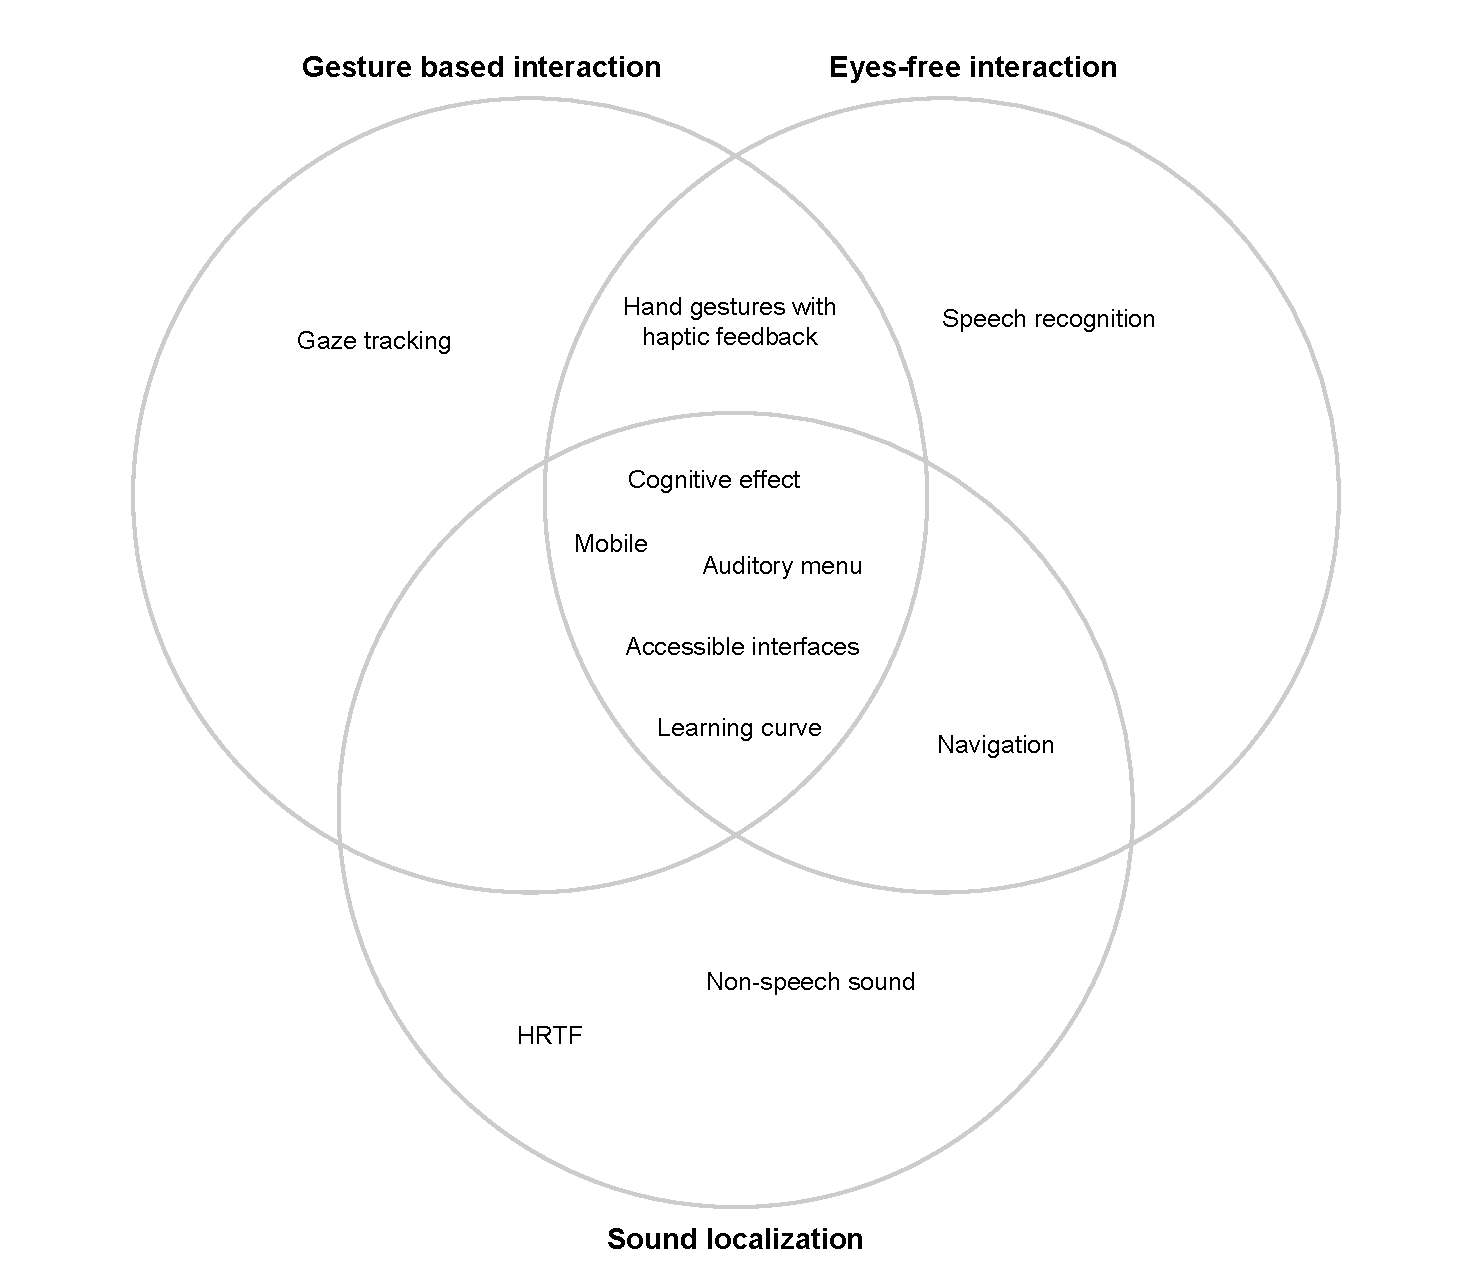
\includegraphics[width=\textwidth,height=\textheight,keepaspectratio]{./Figures/venn-diagram.pdf}
		\rule{35em}{0.5pt}
	\caption[Venn diagram]{A comparison of thesis topics}
	\label{fig:Venn}
\end{figure}

\subsection{Eyes-free interaction}
Several work on both audio \cite{kajastila_eyes-free_2013,bonner_no-look_2010,brewster_multimodaleyes-freeinteraction_2003,zhao_earpod:_2007,vazquez-alvarez_eyes-free_2011} and haptic \cite{pasquero_haptic_2011,pielot_tactile_2011} displays use the term eyes-free which refers to controlling the state of a system without visual attention. This kind of interaction has shown to be desirable in some situations \cite{oakley_designing_2007,yi_exploring_2012} and even improve efficiency compaired to traditional visual displays \cite{zhao_earpod:_2007}.

% visual competition, concentration
One of the main motivations behind this eyes-free use is to design interfaces that do not compete with the users visual attention. That is this "visual competition" could introduce risks when people are on the move e.g. travelling in traffic. In these situations a vital factor is to minimize the amount of distraction for interaction modes \cite{pascoe_using_2000}. Eyes-free interfaces can keep the users visual attention on the road while driving \cite{sodnik_user_2008} or walking around in the city \cite{vazquez-alvarez_eyes-free_2011}.

% visual display problems
Much of the interfaces work in wearable computing tends to focus on visual headmounted displays \cite{barfield_fundamentals_2000} e.g. Google Project Glass. But not only as mentioned does visual displays occupy the users visual attention, they can also be obtrusive and hard to use in bright daylight \cite{geelhoed_safety_2000}. Another disadvantage with visual displays is that their power consumption is high i.e. they drain a mobile device battery and they are expensive. By using eyes-free interfaces it is possible to use cheaper and less power consuming hardware.

\subsection{Head gestures}
There exists different kinds of systems when it comes to controlling an application with head gestures.

\subsection{Spatial sound}
(Spatial audio, Head Related Transfer Function)...\\
Good reference for 3d sound \cite{begault_3dd_1994}

William W. Gaver, a pioneer in audio interfaces, has explored several aspects of using sound in interfaces including the intuitiveness of presenting complex information to users in the form of audio \cite{gaver_sonicfinder:_1989}. Similarly Graham explores the advantages in reaction time when using ”auditory icons” \cite{graham_use_1999}. In \cite{gaver_auditory_1986} Gaver presents the use of spatial sound icons. In doing so, he draws forward the unutilized potential of creating natural interaction through spatial audio.

Kajastila and Lokki has done a user study comparing auditory and visual menus controlled by the same free-hand gestures where the majority of the participants felt that an auditory circular menu was faster than a visual based menu \cite{kajastila_interaction_2013}.

Work has shown that non-speech audio is effective in improving the interaction with mobile devices \cite{pirhonen_gestural_2002, sawhney_nomadic_2000}.

By compairing visual and audio feedback when pushing buttons on the same GUI, Brewster showed that it was difficult for users to devote all their visual attention to an interface while walking, running og driving and that the interaction workload decreased with audio feedback \cite{brewster_overcoming_2002}.


\section{Related work}
Based on the research areas and topics mentioned this section presents the specific related works in these areas and finally a sum up and comparison of the properties of the related works and this thesis.

% closely related to my project
Brewster et al. showed that novel interaction techniques based on sound and gesture can significantly improve the usability of a wearable device in particular under "eyes-free" mobile conditions and that head gestures was a successful interaction technique with egocentric sounds the most effective \cite{brewster_multimodaleyes-freeinteraction_2003}.

\subsection{Summing up: Project focus}
Table: Summing up references that handles specific research areas...














